\begin{figure*}[t]
  \centering
  \subfloat[$e{=}1\%$, exact matching]{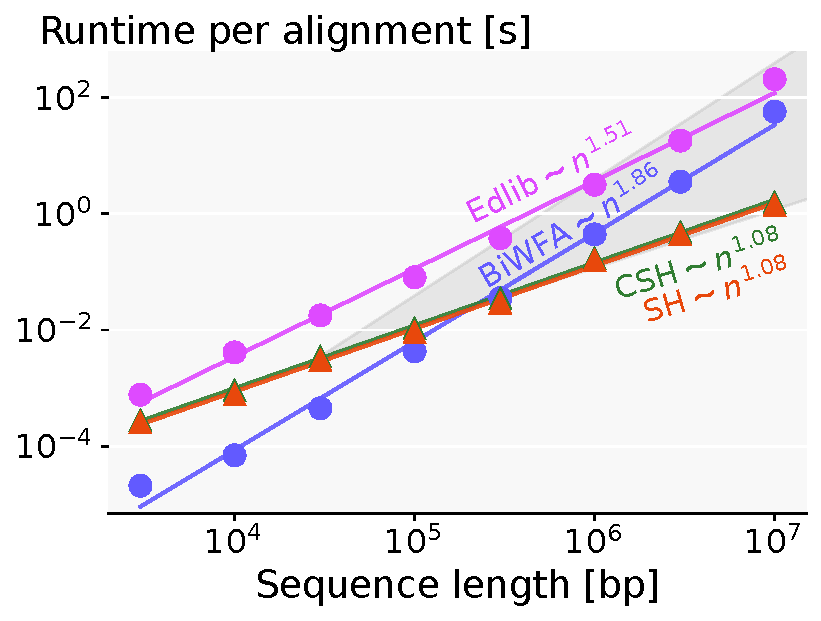
\includegraphics[width=0.4\linewidth]{imgs/fig4/tools_e0.01_labels.pdf}
  \label{GLOBALfig:scaling-n-1}}
  %\hfill
  \subfloat[$e{=}5\%$, exact matching]{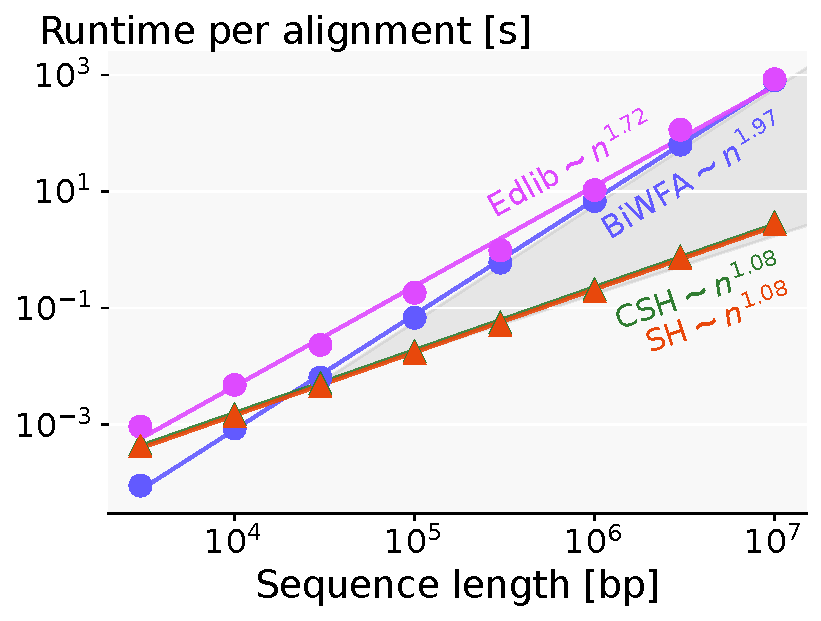
\includegraphics[width=0.4\linewidth]{imgs/fig4/tools_e0.05_labels.pdf}
  \label{GLOBALfig:scaling-n-5}}\\
  %\hfill
  \subfloat[$e{=}10\%$, inexact matching]{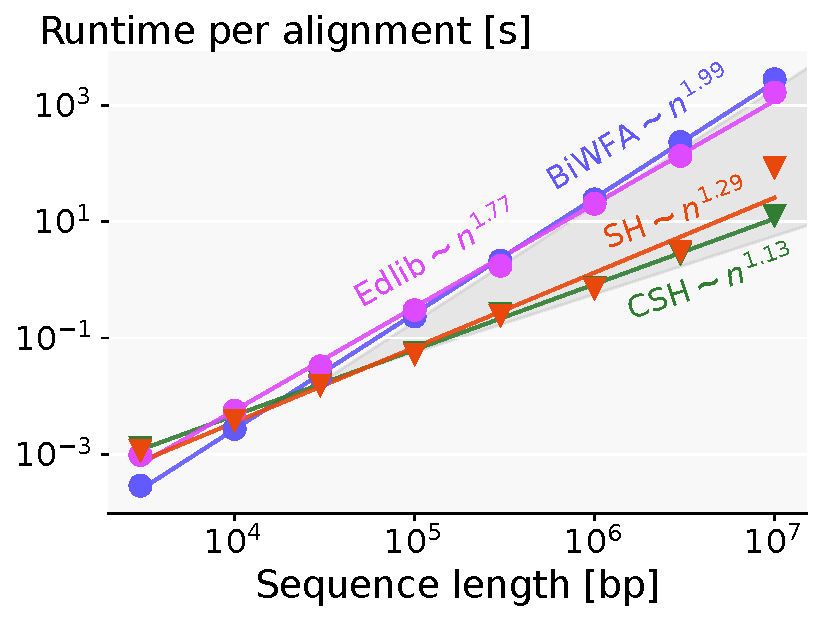
\includegraphics[width=0.4\linewidth]{imgs/fig4/tools_e0.1_labels.pdf}
  \label{GLOBALfig:scaling-n-10}}
  %\hfill
  \subfloat[$e{=}15\%$, inexact matching]{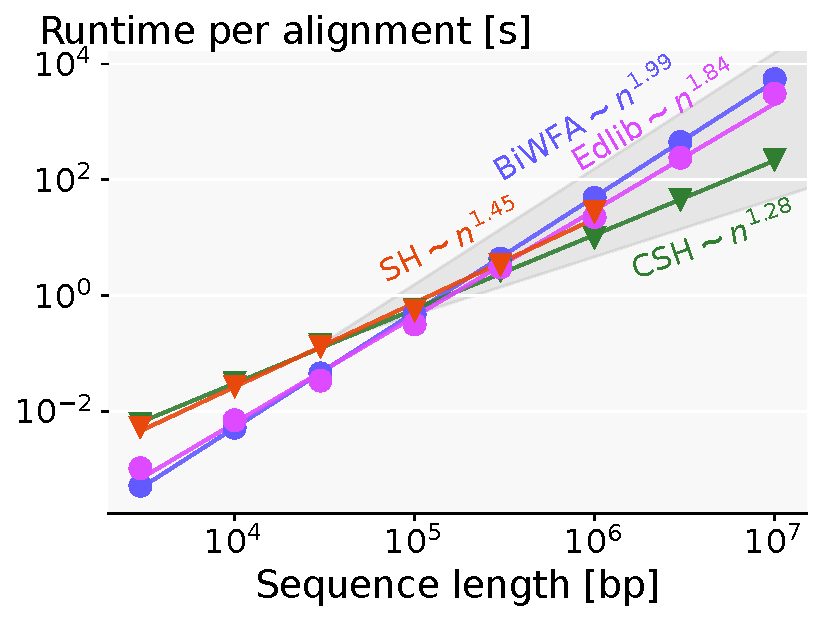
\includegraphics[width=0.4\linewidth]{imgs/fig4/tools_e0.15_labels.pdf}
  \label{GLOBALfig:scaling-n-15}}

  \caption[Runtime scaling with sequence length (multiple error rates)]{Log-log
    plots of the runtime for aligning \textbf{synthetic sequences} of increasing
    length for \astarpa \sh~(\SH), \astarpa \csh~(\CSH), \edlib~(\edlibsymbol)
    and \wfa~(\wfasymbol). The slopes of the bottom (top) of the dark-grey cones
    correspond to linear (quadratic) growth. For $e{\leq} 5\%$,
    \SH~(\shsymbolsq) and \CSH~(\cshsymbolsq) use $k{=}15$, $r{=}1$. For $e{\ge}
    10\%$, \SH~(\shsymbol) and \CSH~(\cshsymbol) use $k{=}15$, $r{=}2$. The
    missing data points for \SH at $e{=}15\%$ are due to exceeding the memory
    limit ($\qty{30}{GB}$). Each runtime is the average over $\lfloor 10^7 / n
    \rfloor$ alignments.}
  \label{GLOBALfig:scaling-n}
\end{figure*}
